\documentclass{article}
\usepackage[UTF8]{ctex}
\usepackage{geometry}
\usepackage{multirow}
\usepackage{natbib}
\geometry{left=3.18cm,right=3.18cm,top=2.54cm,bottom=2.54cm}
\usepackage{graphicx}
\pagestyle{plain}	
\usepackage{setspace}
\usepackage{enumerate}
\usepackage{caption2}
\usepackage{float}
\usepackage{datetime} %日期
\renewcommand{\today}{\number\year 年 \number\month 月 \number\day 日}
\renewcommand{\captionlabelfont}{\small}
\renewcommand{\captionfont}{\small}
\begin{document}

\begin{figure}
    \centering
    
\includegraphics[width=8cm]{upc.png}

    \label{figupc}
\end{figure}

	\begin{center}
		\quad \\
		\quad \\
		\heiti \fontsize{45}{17} \quad \quad \quad 
		\vskip 1.5cm
		\heiti \zihao{2} 《计算科学导论》个人职业规划
	\end{center}
	\vskip 2.0cm
		
	\begin{quotation}
% 	\begin{center}
		\doublespacing
		
        \zihao{4}\par\setlength\parindent{7em}
		\quad 

		学生姓名:\underline{\qquad  杨汶昊 \qquad \qquad}

		学\hspace{0.61cm} 号:\underline{\qquad 1907010308\qquad}
		
		专业班级:\underline{\qquad 计科1903 \qquad  }
		
        学\hspace{0.61cm} 院:\underline{计算机科学与技术学院}
% 	\end{center}
		\vskip 1.5cm
		\centering
		\begin{table}[h]
            \centering 
            \zihao{4}
            \begin{tabular}{|c|c|c|c|c|c|c|c|c|}
            % 这里的rl 与表格对应可以看到,姓名是r,右对齐的;学号是l,左对齐的;若想居中,使用c关键字。
                \hline
                \multicolumn{5}{|c|}{分项评价} &\multicolumn{2}{c|}{整体评价}  & 总    分 & 评 阅 教 师\\
                \hline
                自我 & 环境 & 职业 & 实施 & 评估与 & 完整性 & 可行性 &\multirow{2}*{} &\multirow{2}*{}\\
                分析& 分析& 定位 & 方案 & 调整 & 20\% & 20\% & ~&~ \\\            
                10\% & 10\% & 15\% & 15\% & 10\% & &  &~ &~\\
                \cline{1-7} 
                & & & & & & & ~&~ \\
                & & & & & & & ~&~ \\
                \hline      
            \end{tabular}
        \end{table}
		\vskip 2cm
		\today
	\end{quotation}

\thispagestyle{empty}
\newpage
\setcounter{page}{1}
% 在这之前是封面,在这之后是正文
\section{自我分析}
	% 自我分析即对自己进行全方位、多角度的分析,目的是认识自己、了解自己。只有认识了自己,才能对自己的职业做出正确的选择,才能选定适合自己发展的职业生涯路线,才能对自己的职业生涯目标做出最佳抉择。\par
	% 自我分析包括:\par
\subsection{自然条件}
	我是一个18岁的男生,身体素质较好具有较好的耐力、优秀的柔韧性、较为壮实的身材,健康状况处于亚健康属于易生病的人群,我认为这种相互矛盾的状况是有以下几点造成,一方面我小学、中学经常体育锻炼打下了良好的基础,另一方面高中生活较少的课外时间和学习压力造成部分心理焦虑使得我的免疫力较中小学下降成为易感人群,同时在目前大学生话很少参加经常性、剧烈的体育运动也是一个重要原因。我的故乡在山东省潍坊市昌邑县,现在在大学生活暂居山东青岛市。\par 
% 性别、年龄、身体条件、健康状况、居住城市等\par
\subsection{性格分析}
	性格上略微内向,不太擅长与陌生人打交道。有时候看似勇敢,但实则比较鲁莽。面对事情、考虑问题不够全面,比较缺乏个人主见,对于问题认识比较浅薄。脾气温和,很少生气,不太擅长表达自己的情感。不喜欢评价别人,尊重别人的意愿,不喜欢强迫别人,有时候显得比较孤冷。做事情有时候比较僵硬死板,过于强调要求规则。对于别人的求助,总是尽自己所能出一份力。内心略争强好胜,面对优秀于自己的人会有所失落,内心焦虑。\par
\subsection{教育与学习经历}
	小学就读于昌邑市第一实验小学,中学就读于昌邑市实验中学和峻青中学,高中就读于昌邑市第一中学。此外,课外自初中开始学习信息学奥林匹克竞赛曾在2016、2017获得山东赛区联赛二等奖和一等奖。从小学到初中学习过书法兼修软笔硬笔,曾获得过硬笔八级的好成绩。\par
\subsection{工作与社会阅历}
	由于家庭认为读书对于孩子的我是最重要的任务,同时我也不喜欢和外人打交道,且我也不知道和陌生人怎样聊天获得共同话题,因而我很少和外人打交道。所以对于社会阅历我自认为十分浅薄,缺乏有效的沟通交流能力。尤其是和较自己年龄大的长辈、陌生人交流时显得紧张窘迫,不知道如何是好。比如购物时,明明很简单的口算价格问题,经常算不对,甚至算半天。\par
\subsection{知识、技能与经验}
	精通C++,了解且能使用多种数据结构和算法。对于Java、Python略懂一点。能较为熟练地使用html语言编写网页。可以写一手好字。对于计算机的各种基本知识略懂。简单掌握Latex的使用,能用剪辑软件对视频剪辑、制作电子相册。\par
\subsection{兴趣爱好与特长}
	热衷于学习新的知识,喜欢尝试探索使用各种软件,对于C++编程有所特长,喜欢并在向别人学习篮球。对于自己喜欢的能沉浸其中,对于网络攻防存在较大的兴趣。喜欢阅读网络文学小说(目前不经常读)。课外喜欢偶尔玩玩游戏,看看公众号。\par
\section{环境分析}
% 环境分析主要是评估周边各种环境因素对自己职业生涯发展的影响。每一个人都处在一定的环境之中,职业发展必然要受到所处环境的影响,只有充分了解和把握所处环境的现状、特点、发展变化趋势,才能做到在复杂的环境中避害趋利,使你的职业生涯规划具有实际意义。\par
% 环境分析包括:\par
\subsection{社会环境分析}
	\noindent\textbf{一、政治形势}\par
	我国是一个一党专政国家,中国共产党作为世界第一大党,总人数超过了9000万甚至比一些小国家总人数还要多,同时对军队掌握绝对的领导。无论从软实力还是硬实力,中国共产党都占据绝对的优势。同时,我党具有强大的组织力和凝聚力,具有强大的管理能力。由于,政府、司法等部门要求具有坚定的政治立场势必在行政、司法方面具有浓厚的政治色彩,简而言之可以说具有政治优先。对比同时期的香港,执法人员因与暴徒发生冲突采取了不当措施被判为有罪这就是一个典型的法治优先的例子,在我们看来甚至有些不能理解。而政治优先保障了国家政策可以被高效的贯彻落实,这也是我国近代以来取得重大飞跃的重要原因之一。\par
	\noindent\textbf{二、经济形势}\par
	目前我国具有世界上最为庞大的市场,14亿人口,约占全球总人口的四分之一,具有巨大的发展潜力。同时,我国是世界上唯一一个建成门类齐全、独立完整的现代工业体系的国家。自改革开放以来,我国经济持续高速增长现已成为世界第二大经济体,市场活力较强。但同时,一些产业存在产能过剩、企业间恶性竞争的问题。在高精尖领域,我国还普遍存在受发达国家科技制约的诟病,这些也是我国经济发展的新一轮增长点。\par
	\noindent\textbf{三、就业形势}\par
	目前我国经济面临下行压力,就业形势不容乐观,普遍面临就业压力的的难题。同时,随着教育的普及和发展,本科生的学历已经不再像过去那么吃香,高学历文凭正在变得越来越普遍。而现阶段各大互联网企业纷纷裁员,进一步加剧了就业压力。对于中小型企业的竞争压力增大,随着互联网企业的不断洗牌,目前在各个领域各巨头占据主导地位,利用合并、入股、投资中小企业不断巩固和扩大自身影响力,优化自身结构淘汰冗余人力。\par
\subsection{家庭环境分析}
% 婚姻状况、经济状况、家人期望、家族传统等。\par
	\noindent\textbf{经济状况:}\par 
	对于我的家庭而言,母亲为教师、父亲是工人还要赡养我和爷爷,按照网上的标准甚至不算中产阶级,属于低收入群体。因而对于我个人来说,如果选择创业势必对家庭造成很大的经济和心理压力。对于家人来说,他们更倾向于我选择一份稳定而又体面的工作。对于我爷爷那一辈,他具有较为强烈的乡土情结,舍不得离开故土,也在某种程度上或深或浅地影响了我。而对于我的家族来说我姑和姑父都是公务员具有较为广阔的视野。同时我大爷在国外生活工作的经历也拓宽了我的视野。
\subsection{职业环境分析}
% 行业现状及发展趋势;职业的工作内容、工作要求、发展前景等。\par
	互联网的热潮已经不像过去那么火热,在2015-2017年可以说是互联网投资的热潮,许多实业发家的老板,看到互联网很火想进来试试,在持续投资看不到结果后止损停止,对互联网投资变得谨慎起来。许多互联网企业在通过裁员、减少招聘缩减人力,企图留存资金。而对于一些顶级大厂如BAT等也“不稳定”,京东对10\%总裁级别以上的高管进行末位淘汰,网易方面披露也在进行“结构性优化”。总体来说,就业大环境不容乐观。 \par 
	\begin{figure}[h!]
	\centering
	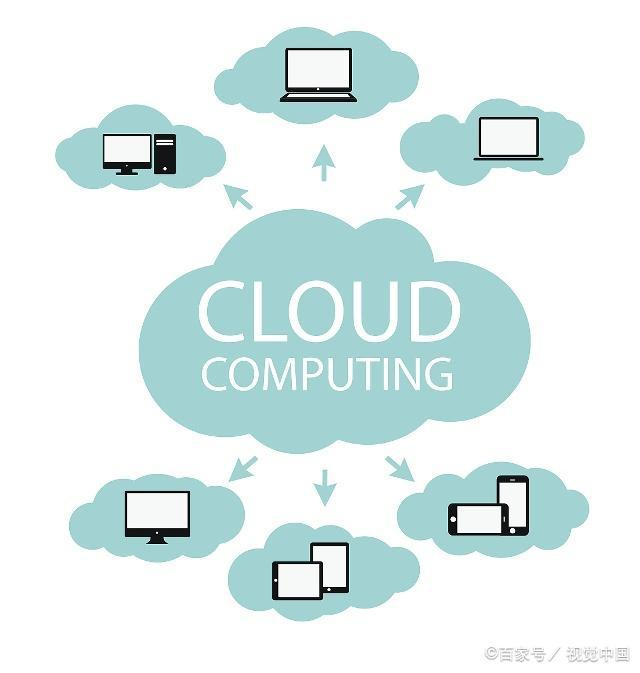
\includegraphics[scale=0.5]{cloud.jpeg}
	% \caption{The Universe}
	% \label{fig:universe}
	\end{figure}
	现在市场就业压力随然增加,但对于人才的渴求也在不断增长,就当前互联网领域薪资排行“云计算、大数据、unity游戏”平均薪资排行前三,尤其是云计算领域的平均年薪已经达到了40万左右!虽说这三个行业薪资排行较高,但是对个人能力要求也是非常高的。这在一定程度上反映了对人才的需求。
	

% \subsection{地域与人际环境分析}
% 工作城市的气候水土、文化特点、发展前景;人脉与人际关系等。\par
% \par 
% 图片插入的样例:\par
% \begin{figure}[h!]
% \centering
% 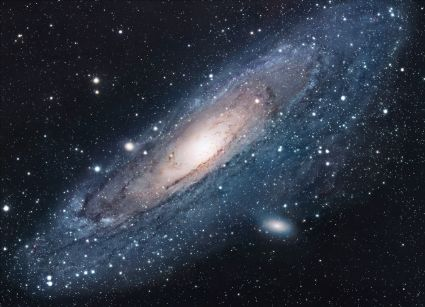
\includegraphics[scale=1.7]{universe}
% \caption{The Universe}
% \label{fig:universe}
% \end{figure}



\section{职业定位}
% 在准确地对自己和环境做出了分析之后,确定适合自己行业和有实现可能的职业发展目标。职业定位时要注意与自己的自然条件、知识背景、技能特长、性格特点、兴趣爱好是否匹配,考虑与自己所处的环境是否相适应。职业定位决定了职业发展中的行为和结果,是制定职业生涯规划的关键,应当科学合理,具有可行性。\par
% 职业定位包括:\par

\subsection{行业领域定位与理由}
	对于未来,我认为大数据云计算、物联网、超级计算机、物联网、区块链的应用前景将非常广泛,甚至可以成为计算机产业的主导产业。然而关于他们的应用,安全问题无疑非常突出,尤其是物联网领域现阶段可以说是“裸机”,一点安全防范也没有,如果有人心怀不轨,势必造成极大的危害。所以,对于网络安全领域,我认为是前景非常光明的。并且,对于我个人来说,成为一名黑客是我小时候的梦想。\par
\subsection{职业岗位起点定位与理由}
	\begin{figure}[h!]
	\centering
	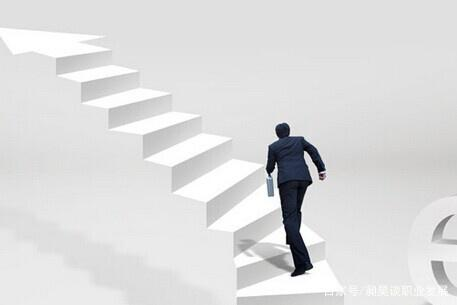
\includegraphics[scale=0.6]{up.jpeg}
	% \caption{The Universe}
	% \label{fig:universe}
	\end{figure}
	\noindent\textbf{起点:}为中企业的渗透测试工程师、网络安全工程师。\par
	\noindent\textbf{理由:}中型企业事务较大型企业较少,可以有更多的空余闲暇时间为自己增值,学习技术。因为我自身出身于计算机科学与技术专业,对于相关的知识较为薄弱,所以可以从基础做起。
\subsection{职业目标与可行性分析}
	关于渗透测试的相关知识我认为和黑客是不谋而合的,所以学习路线参考下页图\par
	\begin{figure}[h!]
	\centering
	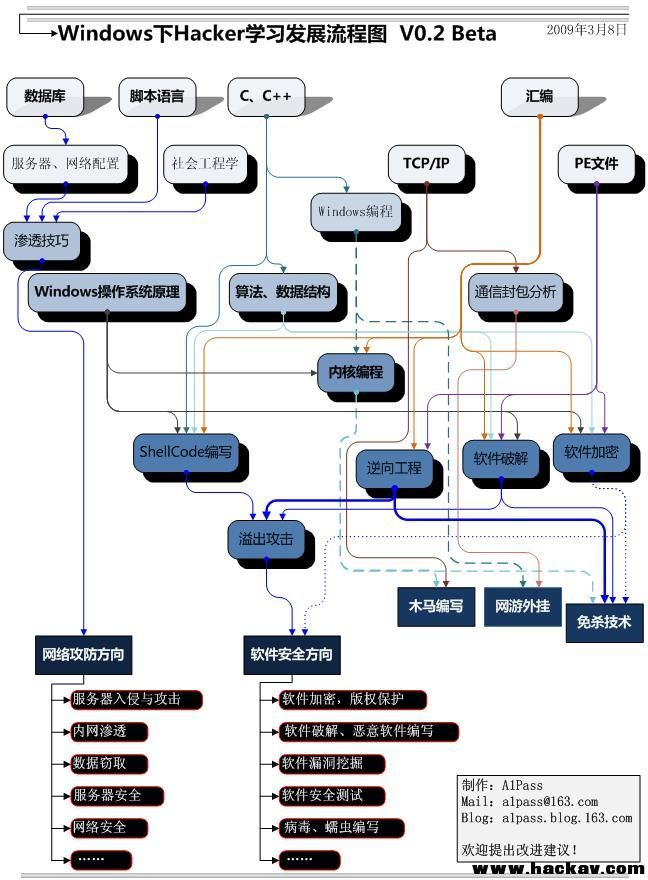
\includegraphics[scale=0.4]{growing.jpg}
	% \caption{The Universe}
	% \label{fig:universe}
	\end{figure}

% 成果目标、经济目标、能力目标、职务目标等。\par 
\begin{itemize}
	\item 在大学四年
		\begin{enumerate}[(1)]
		\item 首先对于学习,具有扎实的数理基础。
		\item 参加网络攻防社团了解更多的相关知识。
		\item 参加CTF比赛,学以致用。
		\item 具有阅读外文资料的能力。
		\item 提升自我沟通能力。
		\end{enumerate}
	\item 中长期目标(5-10年)。
		\begin{enumerate}[(1)]
		\item 跟踪最新前沿技术新闻。
		\item 负责渗透测试工作,进行安全攻击行为的分析及跟踪,报告编写。 
		\item 参与项目实施中涉及的其他安全评估、应急处置等安全技术工作。
		\item 进行漏洞验证及协助整改安全方案,提供安全检测 。
		\item 可以独立完成相关咨询项目信息安全研究报告、安全技术研究 。
		\item 获得有安全和网络相关证书,如CISSP、CISA、CISP 、CCNP、CCIE等认证。
		\item 了解常见的操作系统(LinuxWindows),熟悉shell命令。
		\item 能够阅读一种或多种编程语言,可以进行常见漏洞的代码分析。
		\item 了解常见的端口特征,并能根据banner快速判断可能的漏洞类型。
		\end{enumerate}
\end{itemize}
% 这里是简单列表的样例:(如果需要标号自定义或者自动标记数字序号,请自行搜索语法)
% \begin{itemize}
%     \item 简单的列表结构 
%     \item 如这里所示
%     \item 此处仅为样例
%     \item 按需修改和使用
% \end{itemize}


\section{实施方案}
% 在明确了职业定位后,要制定实现职业生涯目标的行动方案,不付诸行动,职业目标只能是一种梦想。实施方案是实现职业目标的保证,尽量考虑周全、具有可操作性。\par
% 实施方案可以从以下角度考虑:\par
	\begin{enumerate}[1、]
		% \item 如何利用现有条件和自身优势以实现职业生涯目标。
		\item 对于我个人来说,我认为坚韧、勤奋、具有较强的责任和对它感兴趣感是我的优点,加之学校提供了网络安全平台,所以可以通过网络学习相关技术和知识。
		% \item 如何克服缺点、弥补不足、增长知识、提高能力以实现职业生涯目标。
		\item 涉世不深,缺乏社会经验,性格略微内向,社交圈较窄,不具有个人深度思考的能力,针对他们可以在平常生活中刻意克服,强化学习。
		% \item 如何处理人际关系和发展人脉以实现职业生涯目标。
		\item 调整心态,时刻以新人自居,认真向前辈学习,同时多多请教大牛,通过体育、聊天等方式广泛交友。
		% \item 如何处理工作与家庭、生活的关系以实现职业生涯目标。
		\item 工作是为了生存,而家庭是生活,不能为了生存破坏了生活,积极面对压力化压力为动力。
		% \item 如何处理释放工作压力、保证身心健康以实现职业生涯目标。
		\item 参加体育运动如篮球、羽毛球、定向越野等缓解压力,陪伴家人举办家庭活动,和朋友外出旅游等。
	\end{enumerate}
\par 
% 表格插入样例(三线表):\par
%单元格怎么写?参考第一页打分的表格

% \begin{table}[h]
% 	\centering
% 	\caption{这是科学系的花名册}
% 	\begin{tabular}{rl}
% 		% 这里的rl 与表格对应可以看到,姓名是r,右对齐的;学号是l,左对齐的;若想居中,使用c关键字。
% 		\hline
% 		姓名 & 学号 \\
% 		\hline
% 		张三 & 190704xxxx+++ \\ 
% 		李四 & 190704yyyy \\
% 		王二五 & 190704zzzz\\
% 		\hline
% 	\end{tabular}
% 	\label{table1}
% \end{table}
\section{评估与调整}
	\begin{figure}[H]
	\centering
	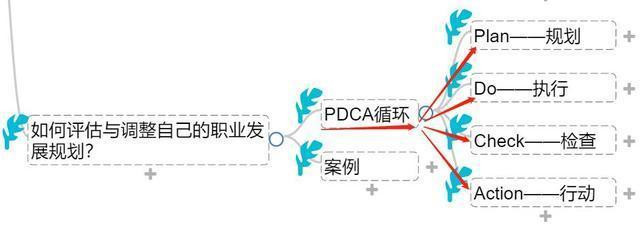
\includegraphics[scale=0.6]{arrange.jpg}
	% \caption{The Universe}
	% \label{fig:universe}
	\end{figure}
% 由于影响职业生涯规划的因素很多,且大都处于动态变化之中,因此职业生涯规划应定期评估,并根据影响因素的变化和实施结果的情况及时作出调整,这样才能保证其行之有效。\par 
\subsection{评估时间}
	% 可以选择每学期评估一次、每学年一次、三年评估一次。\par
	对于每两个星期评估一次,每半学期评估一次,每年评估一次
\subsection{评估内容}
	% 可以从成果目标、经济目标、能力目标、职务目标等方面总结,确定哪些目标已按预期实现,哪些目标商未达到,对已实现的成果总结经验,对未完成的目标分析原因。\par
	对既定目标是否完成、完成情况如何、在实施时发现了什么问题、遇到了什么困难、剩余地是否现阶段有能力完成
\subsection{调整原则}
	% 应考虑与自身情况的匹配性、与环境的适应性、操作实施的可行性等。\par
	对现阶段难以完成的任务推迟延期,对方向错误的改变策略,剩余任务进行目标设定和规划安排




\end{document}
